\subsection{PSYCHE in detail}
\label{subsec:pureshift__psyche_analysis}

\begin{figure}[ht]
    \centering
    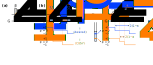
\includegraphics[]{pureshift/psyche_detail.png}%
    {\phantomsubcaption\label{fig:psyche_detail_antizcosy}}%
    {\phantomsubcaption\label{fig:psyche_detail_cosy_suppress}}%
    {\phantomsubcaption\label{fig:psyche_detail_zqc_suppress}}%
    \caption[Detailed analysis of anti $z$-COSY and PSYCHE]{
        A closer look at the mechanism of the PSYCHE PSE.
        \textbf{(\subref*{fig:psyche_detail_antizcosy})} The $\beta$--ZQF--$\beta$ mixing period used in the original anti $z$-COSY experiment. This has a similar action to a JRE, but does not suppress COSY-type coherence transfers from spin $i$ to spin $j$.
        \textbf{(\subref*{fig:psyche_detail_cosy_suppress})} An illustration of how COSY-type artefacts are suppressed by the PSYCHE pulse element. The desired CTP which remains on spin 1 is rephased by the gradients, but the COSY CTP is dephased.
        \textbf{(\subref*{fig:psyche_detail_zqc_suppress})} An illustration of how zero-quantum terms are suppressed by the PSYCHE element through spatial averaging: in each slice of the sample (highlighted in blue and orange), the zero-quantum terms are allowed to evolve for a different duration.
    }
    \label{fig:psyche_detail}
\end{figure}

The anti $z$-COSY experiment utilises a $\beta$--zero-quantum filter (ZQF)--$\beta$ mixing period (\cref{fig:psyche_detail_antizcosy}), where $\beta$ is a small angle, typically \ang{10} to \ang{20}.
The role of the ZQF\autocite{Thrippleton2003ACIE} is to remove terms such as $I_{1-}I_{2+}$ between the two $\beta$ pulses, retaining only population terms such as $I_{1\alpha}I_{2\alpha}$.
The CTPs which this mixing period selects for ultimately give rise to peaks which lie perpendicular to the main diagonal of the spectrum.
In an elegant paper, Pell et al.\autocite{Pell2007MRC} showed that by isolating the diagonal peaks of a 2D anti $z$-COSY experiment and taking the \ang{45} projection of these, a pure shift spectrum could be obtained.
Here, we will go one step further and consider the \textit{direct} use of this element as a JRE: this will reveal some problems which are neatly taken care of by the PSYCHE experiment.

We first need to introduce how the basis operators $\{I_+, I_-, I_\alpha, I_\beta\}$ evolve under a hard pulse (applied along the $x$-axis) with flip angle $\beta$:
\begin{align}
    I_{\pm} &\xrightarrow{\beta I_x} c^2 I_{\pm} + s^2I_{\mp} \pm \frac{\mi S}{2}(I_\alpha - I_\beta) \label{eq:ipm_beta_evolution} \\
    I_{\alpha} &\xrightarrow{\beta I_x} c^2 I_{\alpha} + s^2I_{\beta} + \frac{\mi S}{2}(I_+ - I_-) \label{eq:ialpha_beta_evolution} \\
    I_{\beta} &\xrightarrow{\beta I_x} c^2 I_{\beta} + s^2I_{\alpha} - \frac{\mi S}{2}(I_+ - I_-) \label{eq:ibeta_beta_evolution}
\end{align}
where $S = \sin\beta$, $s = \sin(\beta/2)$, and $c = \cos(\beta/2)$.
Using these formulae, we can show that for a two-spin system (see Pell et al.\autocite{Pell2007MRC} for the equivalent analysis on a three-spin system), the $\beta$--ZQF--$\beta$ element converts the term $I_{1+}I_{2\alpha}$ to
\begin{equation}
    \label{eq:anti_z_cosy_transitions}
    I_{1+}I_{2\alpha} \longrightarrow
    {\underbrace{\frac{1}{2}S^2c^4 I_{1+}I_{2\beta}}_\text{term 1}}
    + {\underbrace{S^2c^2s^2I_{1+}I_{2\alpha}}_{\text{term 2}}}
    - {\underbrace{\frac{1}{4}S^2c^4I_{1\alpha}I_{2+}
    + \frac{1}{4}S^2c^4I_{1\beta}I_{2+}}_{\text{terms 3 and 4}}}
    + \cdots,
\end{equation}
where other terms with different coherence orders have been neglected (on the basis that they can be easily suppressed with bracketing CTP gradients), and terms with higher orders in $s$ have been discarded since $s = \sin(\beta/2) \ll 1$ for small $\beta$.

The first term $I_{1+}I_{2\beta}$, corresponding to the flipping of passive spins only, is the only term we want to see from a JRE.
The second term, $I_{1+}I_{2\alpha}$, corresponds to the case where neither active nor passive spins have been flipped.
In the original anti $z$-COSY work, these give rise to `off-diagonal' peaks which are part of a multiplet on the diagonal, but when projected at \ang{45} generate artefacts around the pure shift peak.
In the context of pure shift NMR, these are called `recoupling artefacts', as they arise from imperfect J-refocusing.
Note that the ratio of recoupling artefacts to desired signal is proportional to $S^2c^2s^2/S^2c^4 = \tan^2(\beta/2)$: using a smaller value for $\beta$ therefore leads to better signal-to-artefact ratios, but also lower overall sensitivity.
The PSYCHE element is similar to the $\beta$--ZQF--$\beta$ element in this regard: it does not suppress the recoupling artefacts, but instead relies on the user choosing a suitable value for $\beta$ such that the artefact-to-signal ratio is tolerably small.
If the sensitivity proves to be insufficient, the flip angle $\beta$ may be increased instead: this leads to a larger artefact-to-signal ratio, but if the sample is not concentrated anyway, it may well be that the artefacts do not rise above the noise level.%

The third and fourth terms, $I_{1\lambda}I_{2+}$ ($\lambda \in \{\alpha,\beta\}$), represent `COSY-type' coherence transfer to a coupled spin.
In the original anti $z$-COSY, these led to crosspeak multiplets at $(\Omega_1, \Omega_2)$, which could be removed by hand before taking the projection.
However, in a pure shift sequence, the peaks arising from these terms cannot simply be removed in the same way.
It is precisely this issue which precludes the $\beta$--ZQF--$\beta$ element from being directly used as a JRE, and motivates the development of the PSYCHE PSE, which \textit{does} suppress these coherence transfers.

To understand how this occurs, we invoke the instantaneous spin-flip assumption.
Each coherence $I_{i+}$ is converted (or `flipped') to a population term $I_{1\lambda}$ at a specific point $\alpha\taup$ after the start of the first chirp, and can be reconverted to a coherence on the same spin $I_{i-}$ at a time $\alpha\taup$ before the end of the second chirp (the blue CTP in \cref{fig:psyche_detail_cosy_suppress}).%
\footnote{Note the change in the sign of the coherence, which differs from the analysis of the anti $z$-COSY experiment. This arises because we are only considering the PSYCHE PSE on its own, \textit{not} the JRE.}
Here, $\taup$ is the duration of the chirp, and $0 < \alpha < 1$.
In this case, the coherence is perfectly rephased by the weak gradient applied during the chirp pulses, since the \textit{time} it experiences these gradients for is the same on both sides of the chirps.
Now, if the $I_{i+}$ term is instead converted to a coherence on a different spin $I_{j-}$, it experiences the gradient for a total duration of $\alpha\taup$ after the start of the first chirp, and also $\alpha'\taup$ before the end of the second chirp (the orange CTP in \cref{fig:psyche_detail_cosy_suppress}).
In general, $\alpha \neq \alpha'$ as spins $i$ and $j$ have different offsets; therefore, this CTP is dephased by the gradients, resulting in suppression of the COSY-type artefacts in the spectrum.

It remains to also consider how the PSYCHE element selects for the population terms between the two spin flips.
Any terms with nonzero coherence order are of course simply dephased by the weak gradient.
However, zero-quantum terms (in homonuclear systems) are not dephased by gradients, and to eliminate them in a single-scan manner, they must be spatially averaged, for example by a ZQF.
It turns out that the PSYCHE element also results in a similar spatial averaging.
Following on from the previous paragraph, the time \textit{between} the spin flips (for the desired pathways, i.e.\ not COSY-type coherence transfer) is given by $2(1 - \alpha)\taup$.
At the same time, the weak gradient induces a range of offsets across the sample, much like in the Zangger--Sterk experiment.
Thus, the offset, and thus the value of $\alpha$, for a given spin depends on which slice it is in; for example, \cref{fig:psyche_detail_zqc_suppress} uses values of $\alpha_1$ and $\alpha_2$ for two different slices (blue and orange).
If zero-quantum terms are present between the spin flips, they evolve during this time and accrue a spatially-dependent phase: summation of these during FID acquisition leads to a cancellation of these terms.
Only population terms such as $I_{1\alpha}I_{2\alpha}$ survive during this, as they do not precess during this time.

The sensitivity of PSYCHE is significantly better than for other methods: depending on the flip angle $\beta$ chosen, $c$ is typically on the order of $0.05$--$0.15$ (see also \cref{fig:fa_dependence_124} for explicit simulations).
Furthermore, it is generally more robust with respect to strong coupling compared to other pure shift methods (artefacts from strong coupling often arise due to unexpected coherence transfer\autocite{Thrippleton2005JMR}, which is suppressed in a similar way to the COSY-type artefacts).
These two factors alone have meant that PSYCHE has enjoyed substantial adoption since its introduction: a large number of 2D experiments utilising PSYCHE decoupling in either $F_1$ or $F_2$ have been developed,\autocite{Foroozandeh2014JACS,Timari2015CEJ,Koos2016ACIE,Sinnaeve2016ACIE,Aguilar2018MRC,Kaltschnee2016JMR,Ilgen2021JMR} notably the PSYCHE-iDOSY diffusion experiment\autocite{Foroozandeh2016ACIE}, where the increased resolution provided by pure shift spectroscopy translates into increased resolution in the \textit{diffusion} dimension as well.
Like the ZS element before it, the PSYCHE element has also been used for the acquisition of absorption-mode 2DJ spectra.\autocite{Foroozandeh2015CC}

Despite this success, PSYCHE suffers from one significant drawback: it cannot be used in a real-time fashion.
The PSYCHE PSE is often said to select active and passive spins in a `statistical' manner: this is because of the $c^2$ and $s^2$ terms arising from the low-flip angle pulses.
What this really means is that we do not care \textit{exactly} which spins are active and which are passive, but that a certain proportion of the spins are active and passive.
Repeated application of the PSE therefore does not select for the same active spins each time, which precludes its application to real-time acquisition.

Although the PSYCHE PSE may appear deceptively simple at first glance, the closer analysis given here (and elsewhere\autocite{Foroozandeh2018CEJ}) clearly shows that its inner workings are anything but.
Along with other ingenious experiments such as the ZQF\autocite{Thrippleton2005JMR}, ultrafast NMR\autocite{Frydman2002PNASUSA,Pelupessy2003JACS,Frydman2003JACS}, and more recently GEMSTONE\autocite{Kiraly2021ACIE}, PSYCHE is a prime example of how \textit{spatiotemporal averaging} and pulsed field gradients can be used to great effect in modern NMR spectroscopy.\autocite{Dumez2018PNMRS}

At the same time, PSYCHE itself is not \textit{perfect}: it does not fully suppress recoupling artefacts, and can only be used in the interferogram mode.
To improve on PSYCHE would therefore entail one of the following:
\begin{enumerate}
    \item increasing the sensitivity (while maintaining purity);
    \item increasing the purity (while maintaining sensitivity); or
    \item developing a pure shift element which is compatible with real-time acquisition while giving comparable sensitivity and purity to PSYCHE.
\end{enumerate}

The sections which follow describe my efforts towards objectives (1) and (2).
